\section{Metodología de Desarrollo Software}
Synaptix selecciona desarrollo iterativo e incremental con gestión de flujo Kanban y controles de desarrollo seguro SSDF de NIST. Kanban aporta políticas y métricas; SSDF incorpora seguridad al ciclo. La elección permite coordinar nueve dominios, integraciones y revisiones compartidas sin declarar equipos dedicados que SD7 no haya dimensionado. El detalle se entrega en el Formulario T-10, \ArchivoTDiez. \parencites[apartados Kanban Practices y Flow Metrics, pp.~3--5]{sd6-kanban}[sec.~2; tabla~1]{sd6-ssdf}

\subsection{Requisitos, flujo y capacidad de construcción}
Cada elemento representa un resultado verificable y conserva requisito T-12, dominio, paquete EDT, etapa, recepción, esfuerzo y responsable. El flujo empieza al seleccionar capacidad autorizada para construir y termina con incremento verificado y expediente. Antes del inicio deben estar disponibles criterios de aceptación, contratos de interfaz, datos de prueba y dependencias. Las funciones transversales no se reconstruyen por cada dominio ni innovación. \parencite[RT-04.04; RT-20.07, pp.~10/35]{sd6-bt}

La Figura~\ref{fig:flujo_desarrollo} resume el flujo de desarrollo y liberación, con corrección y retorno ante fallas. El tablero distingue resultados verificados, pendientes de autorización y liberados; los bloqueados conservan su estado y antigüedad.

\begin{figure}[htbp]
    \centering
    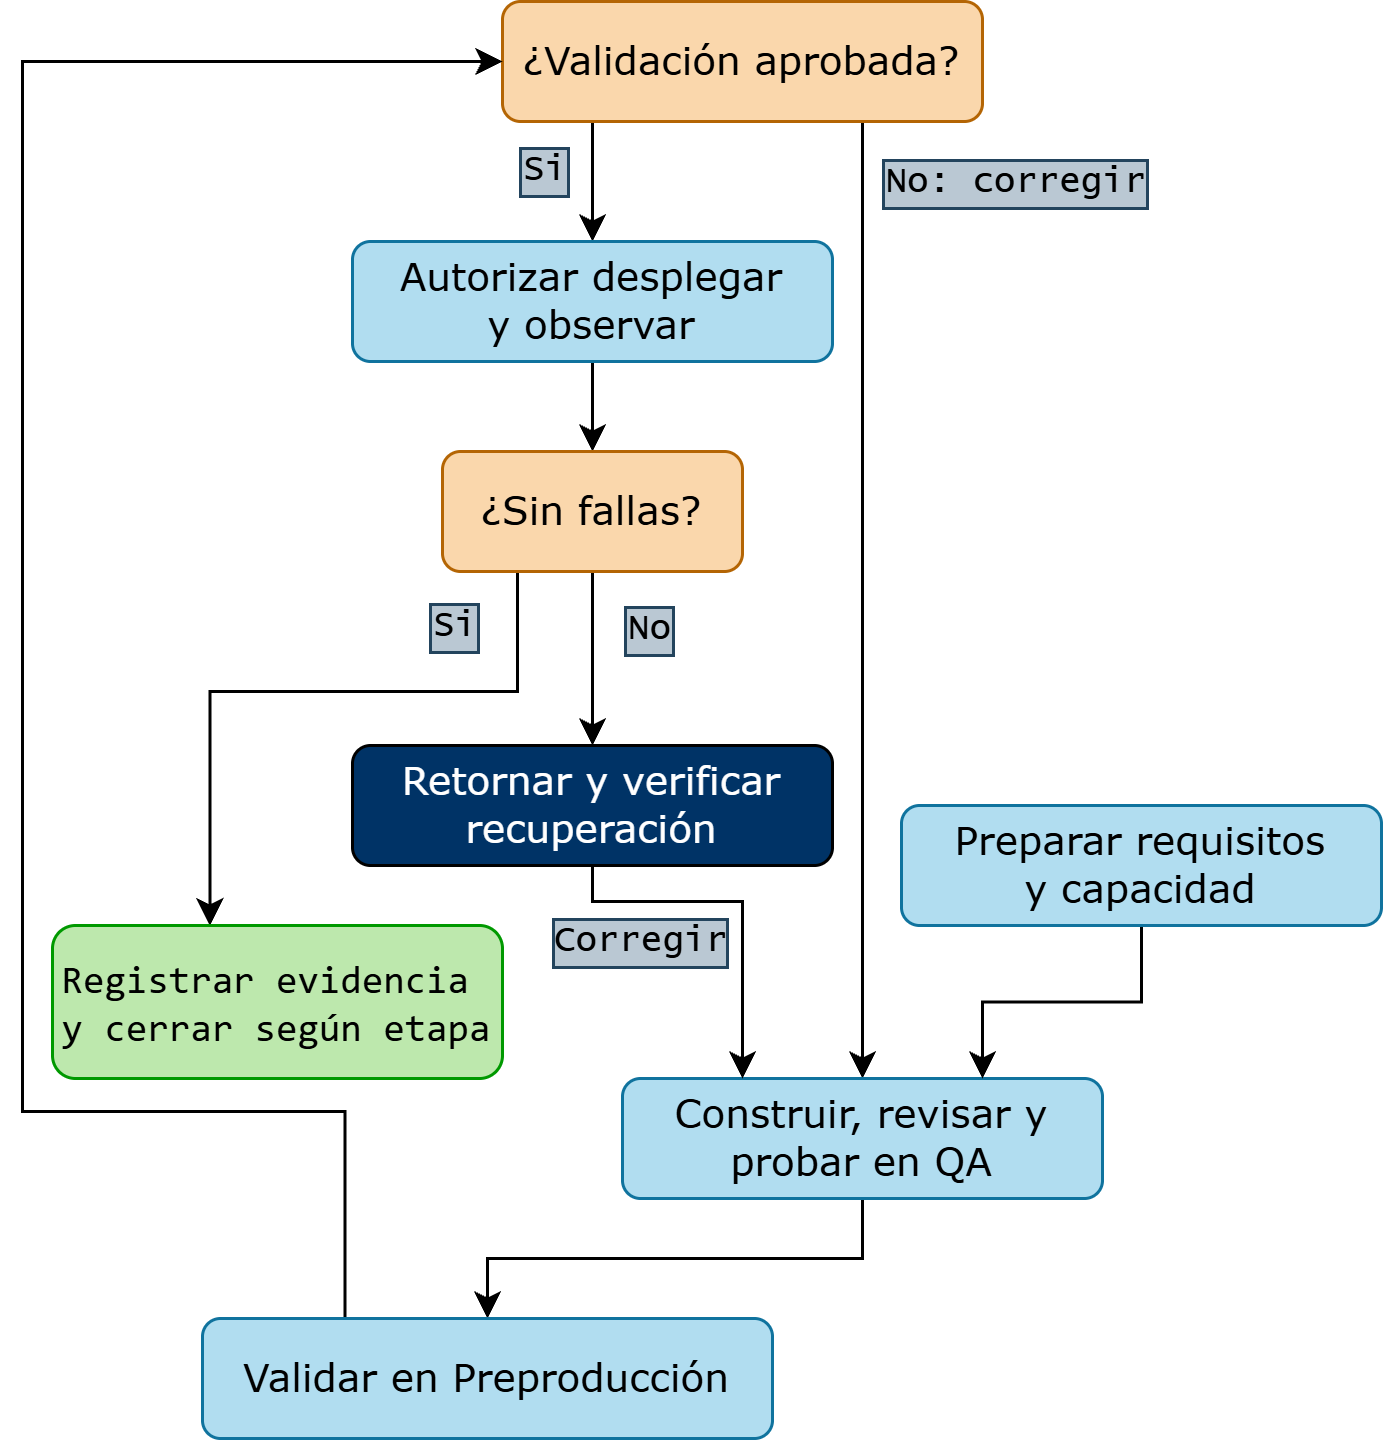
\includegraphics[width=0.55\linewidth]{figuras/F6_2.png}
    \caption{Flujo de incremento y promoción controlada}
    \label{fig:flujo_desarrollo}
    \par\fontsize{9}{12}
\end{figure}

\newpage
Calidad verifica criterios sin asumir horas de construcción. Funcional valida comportamiento, Seguridad los controles y SRE el despliegue y retorno. La Contraparte acepta conforme a T-17. Una demostración no cierra un resultado que incumple la definición de terminado.

La oficina programa reposición y revisión por quincena civil: 1--15 y 16--último día, conservando la unidad de SD7. No son sprints de duración constante. Desarrollo coordina impedimentos diariamente y realiza revisión y retrospectiva al cierre quincenal. Son cadencias propuestas por Synaptix, con horas incorporadas a las asignaciones existentes, sin añadir una sobrecarga general. El trabajo comienza sólo con disponibilidad de ejecución y revisión.

El límite de trabajo en curso depende de capacidad: cada persona ejecutora admite un elemento activo de construcción; cada revisora, uno en revisión; y cada frente habilitado, uno esperando verificación. Un elemento con varias personas cuenta una vez en el tablero y reserva capacidad en todas sus agendas. La restricción cambia con dotación y bloqueos sin retirar suspendidos del conteo. T-10 especifica estados, políticas y excepciones.

\subsection{Arquitectura evolutiva, codificación y deuda técnica}
Arquitectura conserva autoridades funcionales de SD3--SD5, el modelo híbrido e interfaces versionadas. Cada decisión relevante registra requisito, opciones, justificación, impacto en seguridad/datos, prueba y transición. El Comité de Arquitectura la revisa; si modifica el compromiso contractual, pasa además por control de cambios. La evolución mantiene la operación local desconectada y la autoridad de los datos.

El cliente es titular del repositorio Git privado de código, documentación, modelos, configuración e infraestructura, y propietario de los desarrollos específicos desde su creación. Synaptix lo administra con permisos nominativos delegados, sin restringir la titularidad ni el acceso autorizado del cliente. Cada liberación actualiza fuentes y manifiesto reproducible en ese repositorio; SD7 programa además la custodia independiente, actualización semestral y liberación por insolvencia o incumplimiento grave. La política de ramas protegidas de T-10 se aplica a main y release: sin escritura directa, force-push, eliminación ni bypass; revisión independiente ligada al commit y controles obligatorios conformes. LIB-6 1.0 conserva la cadena requisito--incidencia--código--prueba ejecutada--despliegue efectivo, con contratos/esquemas, digest, configuración, resultado y retorno; una aprobación anterior no habilita código nuevo. Los estándares aplican tipado, validación en fronteras, errores explícitos, pruebas de autorización e idempotencia y registros sin datos personales innecesarios. Se utiliza la tecnología seleccionada en SD4; T-10 define recepción y aprobación de dependencias. \parencites[art.~84.1/6, p.~43]{sd6-ba}[RT-04.03/04, p.~10; RT-11.26, p.~24]{sd6-bt}[PS.1; PW.4--PW.8, tabla~1]{sd6-ssdf}

El registro de deuda cuantifica horas, riesgo, componente, causa, prioridad y cierre. Se conserva F24 de SD7: 32 HH mensuales de deuda dentro de 240 HH de las bolsas correctiva, normativa, evolutiva y deuda; $32/(80+48+80+32)=0,1333$, equivalente a 13,33\,\%. El mantenimiento de 24 HH reserva su 20\,\% interno, $24\times0,20=4,8$ HH, para sus propias acciones. Una misma corrección se imputa una sola vez. El denominador de 13,33\,\% es esa capacidad de ingeniería, no todos los turnos de Operación. Desarrollo controla consumo y reducción efectiva mediante pruebas y cambios cerrados. \parencite[RT-21.21, p.~38]{sd6-bt}

\subsection{DevSecOps, ambientes y cadena de suministro}
SD4, tabla Producción y Preproducción: igualdad y diferencias seleccionadas, fija EQ-4 1.0 por componente: topología, versiones y configuración iguales, recursos del escenario ensayado, cuentas/secretos/datos y destinos de prueba propios. T-11 separa el par local y la red del laboratorio del parque productivo. La promoción exige comparación normalizada y pruebas con capacidad y cuotas suficientes a 1,5 veces el peak habilitado; si cambia ese peak, se actualiza y ensaya el mismo perfil en ambos ambientes. Los cinco ambientes de SD4 son Desarrollo, QA, Preproducción, Producción y Recuperación ante desastres, operativos para H3 de E-25. Preproducción conserva topología, versiones y configuración productivas; las diferencias de capacidad se declaran. Los ambientes no productivos usan datos sintéticos o protegidos verificablemente. OpenTofu versiona infraestructura, configuración se externaliza y secretos se obtienen del gestor por ambiente. SEC-ROT-1.0 y GLS-1.0 de SD4 gobiernan rotación automática, revocación y auditoría cloud/local; la configuración conserva referencias y ningún secreto embebido. El mismo digest se promueve sin recompilación. T-10 desarrolla la recepción H3 de los cinco ambientes, la reconstrucción desde código, el reinicio verificable de QA y la conmutación/retorno DR semestrales; el acta con una comprobación fallida impide recibir el hito. \parencite[RT-04.01/02/08/09, pp.~10--11; RT-11.25, p.~24]{sd6-bt}

GitHub Actions coordinará compilación, pruebas y controles: SonarQube para análisis estático y calidad; Trivy para dependencias, imágenes e infraestructura; Gitleaks para secretos; ZAP para DAST autenticado; y Cosign para firma y procedencia. Esta selección conserva la cadena declarada en T-12. T-11 precisará versiones, edición, licencias y compatibilidad. Los workflows y reglas estarán versionados, con acciones y dependencias fijadas a referencias inmutables. El manifiesto registrará herramientas, configuración y huellas utilizadas. Un control ausente, fallido o de otra versión, un secreto detectado o un hallazgo crítico/alto abierto bloqueará el despliegue. La Tabla~\ref{tab:sd6-puertas} resume los controles; T-10 define responsables y verificación. \parencites[RT-04.01--12, pp.~67--69]{sd6-t12}[PO.3/PO.4; PW.7/PW.8, tabla~1]{sd6-ssdf}

\begin{table}[htbp]
\caption{Controles de promoción de una versión}\label{tab:sd6-puertas}
\begin{tabularx}{\linewidth}{L{.24\linewidth}Y L{.23\linewidth}}
\hline
\EncabezadoTabla{Control} & \EncabezadoTabla{Condición de salida} & \EncabezadoTabla{Evidencia}\\\hline
\rowcolor{SynSurface} Construcción & Pruebas sin fallas y cobertura de negocio al menos 70\,\%. & Reporte por commit.\\\hline
Seguridad & Sin hallazgos críticos/altos abiertos para producción. & Análisis y remediación.\\\hline
\rowcolor{SynSurface} Suministro & SBOM, firma, procedencia y digest verificables. & Manifiesto de versión.\\\hline
Aceptación & Pruebas, retorno y autorización completos. & Expediente T-17/T-18.\\\hline
\end{tabularx}
\FuenteTabla{Bases Técnicas Transversales: RT-04.05/11, pp.~10--11; RT-11.20/22--27, p.~24; cap.~20, pp.~34--35. Aplicación al diseño de SD4.}
\end{table}
La cobertura divide líneas ejecutables de negocio ejercitadas por el total de esas líneas. Reporte ausente bloquea; no se excluyen funciones para elevar artificialmente el porcentaje. Seguridad exige revisión de diseño y pruebas adversas, además del análisis automático. Un tercero independiente ejecuta intrusión antes de cada paso a producción y anualmente, con informe íntegro al cliente. \parencite[RT-04.11, p.~11; RT-11.20/22, p.~24; cap.~20, p.~34]{sd6-bt}

La procedencia seguirá SLSA Build L3, versión 1.2: plano de control que genera y firma la atestación separado del código de construcción, aislamiento entre ejecuciones y custodia de claves. Se verifica fuente, parámetros, plataforma autorizada y digest. Una firma aislada no acredita L3; la habilitación comprobará que el build no puede falsificar procedencia ni acceder al material de firma. Se entrega SBOM CycloneDX o SPDX por versión. \parencites{sd6-slsa,sd6-slsa-requisitos}[RT-11.23/24, p.~24]{sd6-bt}

\subsection{Liberación, migración y aceptación}
DEP-6 1.0 de T-10 ejecuta liberación y retorno reproducibles mediante workflows de GitHub Actions y el agente autorizado del Runtime, con plan firmado, estado persistente, pasos idempotentes, comprobación de autoridad HA y paquetes anterior/nuevo disponibles localmente. La autorización precede a la ejecución: ningún paso productivo requiere comandos humanos. Se selecciona azul-verde para aplicación cloud y para slots Podman N/N+1 del nodo local activo: 10\,\% del tráfico cinco minutos, 100\,\% y observación quince minutos, con retorno automático ante falla crítica, SLO incumplido o integridad fallida. El módulo de encaminamiento del Runtime conserva conexiones y drena el ejecutable anterior; sesiones, resultados idempotentes y diario se conservan fuera del slot. Esta promoción compatible no conmuta el primario PostgreSQL ni la IP virtual. T-10 exige ensayo completo EQ-4 antes de cada producción, a 1,5 veces el peak, con peticiones en vuelo, conexiones largas, fallas y retorno, sin pérdidas, duplicados, interrupciones ni plazos incumplidos. El solapamiento mantiene el 40\,\% de reserva local; si no cabe, se redimensiona antes de promover. Son condiciones futuras de recepción, no mediciones ejecutadas. \parencite[RT-04.06/07, p.~11]{sd6-bt}

La actualización secuencial de infraestructura continúa automatizada bajo Pacemaker/Corosync y fencing, sin actualizar ambos nodos a la vez. Sin embargo, un reinicio de nodo o una conmutación de primario, IP virtual, GLS, broker o módulo de encaminamiento puede cortar conexiones: ese camino no demuestra liberación sin interrupción. T-10 declara esta brecha y bloquea esas clases como promoción conforme a RT-04.07 hasta desarrollar y ensayar continuidad de extremo a extremo. Una ventana de mantenimiento, conservación de registros o recuperación dentro del RTO no sustituye ese criterio. \parencite[art.~20, pp.~14--15]{sd6-ba}

Los esquemas PostgreSQL evolucionan por incorporación, transición y retirada, con scripts versionados, originales conservados y convivencia de dos versiones. MIG-6 1.0 de T-10 ejecutará automáticamente el avance y la reversa mediante workflows de GitHub Actions y el agente local autorizado de DEP-6, sin comandos manuales en Producción. Cada ejecución conservará huellas, exclusión mutua entre migraciones sobre la misma base y reporte por paso; los cambios de esquema coordinarán el acceso del escritor según el procedimiento ensayado. Se probarán N/N+1 concurrentes y los hechos nuevos generados durante el retorno. Una migración sin reversa representable y ensayada se bloquea. Antes de retirar estructura irreversible se verifica copia y se ensaya restauración y reaplicación de hechos. Revertir el ejecutable no recupera datos destruidos. La migración histórica y conciliación siguen SD5 y los dos ensayos de SD7. \parencite[RT-04.10, p.~11; cap.~20, pp.~34--35]{sd6-bt}

La gestión, documentación y diseño de pruebas aplican ISO/IEC/IEEE 29119-2:2021, 29119-3:2021 y 29119-4:2021, respectivamente. T-10 vincula cada proceso con su responsable, artefacto y condición de salida; SSDF complementa el desarrollo seguro. Antes de cada paso a producción se comprobarán carga y estrés a 1,5 veces el peak declarado, conformidad WCAG 2.2 AA documentada, seguridad, resiliencia y conmutación real DR. Se añaden aceptación, sincronización y desconexión recinto/terreno conforme al protocolo aplicable. La marcha blanca conserva convivencia, conciliación diaria y umbrales T-18. El acta de cierre precede al cambio oficial de autoridad; recibir evidencias parciales no adelanta producción de mes 16 o 21. Una puerta fallida bloquea el avance y activa la contingencia de SD7, manteniendo calendario y responsabilidades contractuales. \parencites[art.~4.3, pp.~5--6; art.~17.3, pp.~12--13]{sd6-ba}[cap.~20, pp.~34--35]{sd6-bt}{sd6-29119-2,sd6-29119-3,sd6-29119-4}[13.3, pp.~29--30]{sd6-c07}

Se medirán por separado la disponibilidad mensual de las transacciones críticas de extremo a extremo, de al menos 99,9\,\%, y la de los componentes aplicables, de al menos 99,95\,\%. Cada indicador tendrá alcance, método y exclusiones justificadas; cumplir uno no sustituye al otro. El presupuesto transaccional de 0,1\,\% mensual de T-12 regulará los despliegues: agotarlo congelará las liberaciones ordinarias del servicio afectado, sin justificar incumplimientos de componentes. Antes de promover se comprobarán ambos indicadores y la continuidad; disponer de presupuesto no autoriza interrupciones programadas. Las correcciones urgentes seguirán el procedimiento de incidentes autorizado, conservando controles, trazabilidad y restricciones operacionales. \parencites[RNF-DISP-01, p.~50; RT-10.09, p.~105]{sd6-t12}[RT-04.07, p.~11; RT-10.01/06/09, p.~22]{sd6-bt}

\subsection{Medición del flujo y mejora continua}
El tablero registra trabajo en curso, elementos terminados por unidad de tiempo, antigüedad de abiertos y tiempo de ciclo. Comienzo y fin tienen idéntica definición en conteo y decisión. La expectativa inicial de servicio es terminar el 85\,\% de elementos de construcción en veinte días hábiles: objetivo de planificación de Synaptix que se recalibrará con tiempos observados, sin presentarlo como probabilidad demostrada. Retrasos y bloqueos permanecen visibles. \parencite[Definition of Workflow y Flow Metrics, pp.~3--5]{sd6-kanban}

RT-04.12 se instrumenta por servicio con frecuencia de despliegue, tiempo commit--producción, tasa de cambios fallidos y restauración. T-10 declara objetivos y denominadores. Los congelamientos se registran sin borrarlos del tiempo de entrega. Estas métricas no sustituyen disponibilidad, aceptación ni plazos contractuales. Seguridad realizará evaluación inicial y reevaluación anual OWASP SAMM conforme al control de SD4, con evidencias y acciones por práctica; no se declara certificación obtenida. \parencites[RT-04.12, p.~11; RT-11.28, p.~24]{sd6-bt}{sd6-samm}

La retrospectiva quincenal registra mejora, responsable, esfuerzo y comprobación, dentro de capacidad disponible. El expediente final reúne fuente, configuración, pruebas, SBOM, firma, manuales, despliegue, retorno y actas. Así, el cliente puede revisar los resultados y Operación reproducirlos y mantenerlos.
